\section{Control} \label{sec:control}
El sistema de control de nuestro robot fue una de las partes más complejas del proyecto, tanto por la integración de múltiples herramientas como por la interpretación de los modelos dinámicos que definen su comportamiento.

Si bien no pudimos implementar un control completamente optimizado o formalmente validado, se realizaron los siguientes enfoques:

\begin{itemize}
    \item \textbf{Modelo dinámico:} Utilizamos un modelo simplificado del robot (por ejemplo, tipo diferencial o con cinemática holonómica, según el caso) para obtener una aproximación del comportamiento esperado. Esto sirvió como base para definir las señales de control requeridas.
    
    \item \textbf{Controlador básico:} En la práctica, implementamos un controlador proporcional (P) o proporcional-integral (PI), dependiendo de la tarea. Este controlador se aplicó para regular la velocidad lineal y angular del robot, tratando de minimizar el error entre la trayectoria deseada (por ejemplo, obtenida con MATLAB o RViz) y la trayectoria real.
    
    \item \textbf{Simulación en Gazebo:} Validamos de forma empírica el comportamiento del sistema mediante simulaciones en Gazebo, ajustando manualmente los parámetros del controlador para obtener un desempeño aceptable.
    
    \item \textbf{Limitaciones:} A pesar de nuestros esfuerzos, el control del robot no alcanzó un nivel óptimo de precisión ni estabilidad, debido a la complejidad de integrar correctamente el modelo dinámico con las entradas de control en ROS y los sensores simulados en Gazebo.
\end{itemize}

Aunque aún nos falta profundizar en los fundamentos teóricos y matemáticos detrás del control óptimo, este proyecto nos permitió tener un primer acercamiento práctico a los desafíos reales del control de robots móviles. Agradecemos la oportunidad de intentar abordarlo, aun sin una solución definitiva.

\begin{figure}[H]
	\centering
	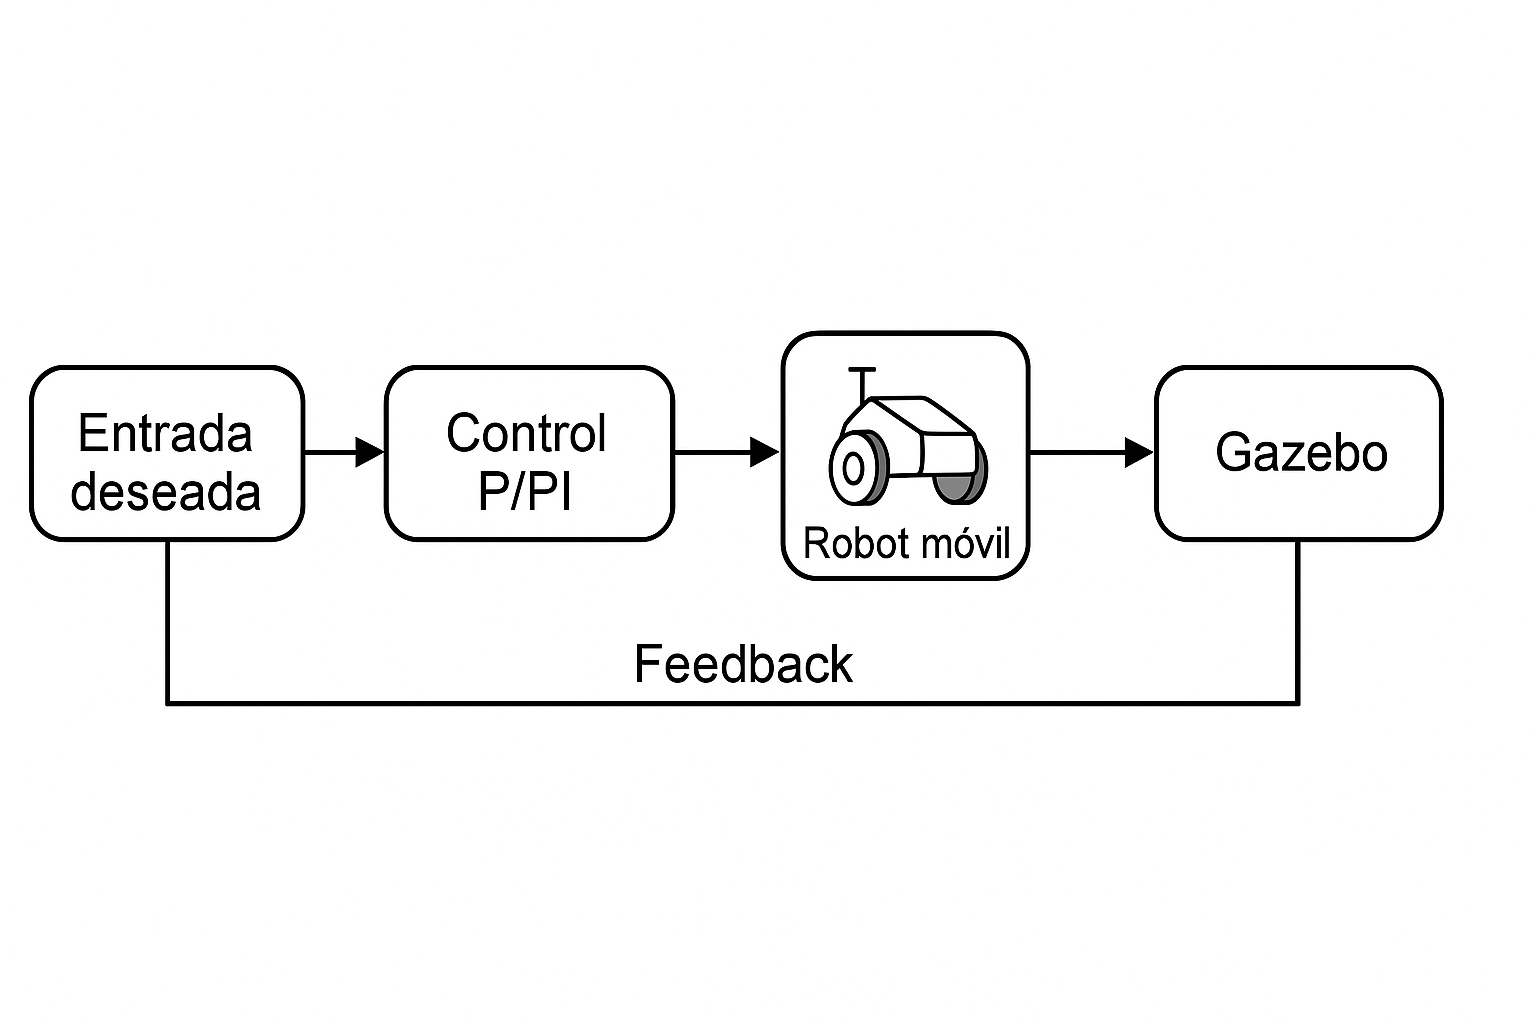
\includegraphics[width=0.5\textwidth]{img/Modelo de Control.png}
	\caption{Modelo de Control}
	\label{fig:Modelo de Control}
\end{figure}